\appendix

\section{Initial Conditions}\label{app:ics}
\subsection{Update to Initial Conditions Code}
The routines to generate the initial conditions of the central and satellite galaxies are descended from the \texttt{MakeNewDisk} code first described in \tocite. This code originally allowed for a Hernquist halo, exponential gas and stellar disk, and Hernquist bulge to be constructed in equilibrium by approximating the distribution function as a Gaussian. This code was recently extended by \citet{2023MNRAS.tmp.2070B} to also allow for the construction of a gaseous halo with a $\beta$-profile which surrounds the disk. This halo is given a rotational velocity which is a fixed ratio of the circular velocity. The interested 

We have made a few modifications to the \citet{2023MNRAS.tmp.2070B} code. First, we have added the ability to vary the value of $\beta$, which was previously fixed to $2/3$. Second, we can now vary the fraction of the gaseous halo's rotational velocity to the circular velocity, which was fixed at $0.4$. The central density of the $\beta$ profile is also chosen differently. We now fix the total mass inside of $R_{200}$. The user now specifies the baryon fraction within $R_{200}$ (nominally the universal baryon fraction), from which the dark matter halo mass and central density are derived. For other details of the setup, we refer the interested reader to \citet{2023MNRAS.tmp.2070B}.

A detailed description of our setup is described in Appendix~\ref{app:ics}. Briefly, for both the central and satellite galaxies we initialize a dual system of both a Hernquist halo as well as a $\beta$-profile. \red{fix: this is confusing}. The haloes are in gravito-hydrostatic equilibrium with themselved. We do not initialize either galaxy with a disk, rather allowing the disk to form self-consistently out of the collapsing profile. This is an attractive setup because it means that the disk-CGM interface as well as the abundance of star particles are formed self-consistently.

For the central galaxy, meant to imitate the Milky Way, we choose a halo mass of $5\times10^{11}\,\Msun$.\footnote{When discussing halo masses in the \texttt{MakeNewDisk} lineage, it is important to remember that a Hernquist profile is chosen such that its profile within the scale radius matches an NFW halo\red{cite} of a certain mass, size, and concentration. This means that the actual mass contained within $R_{200}$ is less than would be contained within an NFW halo, since the Hernquist halo's density drops more quickly than NFW past the scale radius. This is unimportant for studies of the internal structure of galaxies, but in our work this distinction would mean that the given orbits would need to be adjusted.} This is roughly the expected halo mass of the Milky Way at $z\sim2$ from abundance matching\red{cite} in combination with the expected stellar mass-halo mass relation \red{cite}. We allow $\beta$ to be $0.8$ and set the central density to $\sim4.1\times10^{-4}\,\Msun/\pc^3$, such that the baryon fraction within $R_{200}$ is $8\%$. The core radius is set to be $9\,\kpc$, though the resultant galaxy is not very sensitive to the core radius.

For the satellite galaxy, meant to imitate GSE, we choose a halo mass of $\sim2.2\times10^{11}\,\Msun$. We also use a $\beta$ value of $0.8$ and set the central density to $\sim3.5\times10^{-4}\,\Msun/\pc^3$, such that the baryon fraction within $R_{200}$ is $6\%$. The core radius is set to $6.5\,\kpc$, which similar to the central does not have a large impact.

Our setup is not meant to be taken literally as a representation of the evolution of the Universe from $z=\inf$ to $z\sim2$. In particular, we have made manual adjustments to the setup parameters as well as the feedback model in order to arrive at a well-behaved disk after $\sim3\,\Gyr$ of evolution. We experimented with stronger feedback models, but found that higher baryon fractions were required to achieve reasonable stellar masses. This may come from the unrealistic aspects of our setup. In particular, our potential is initially deep, while in the real universe the potential will deepen gradually over time. Thus, a galaxy can form and become self-regulating in a less intense environment than in our setup. We account for this by lowering the baryon fraction to well below the universal value.

\subsection{Orbital Parameters}\label{ssec:orbits}
In this work, we explore a very narrow region of the orbital parameter space, building on the maximum likelihood model from \citet{2021ApJ...923...92N}. We situate the satellite galaxy at a given starting radius $R_0$. Given the symmetry, the satellite is placed on the $x$-axis. 

We then assign a velocity of magnitude $V_0$ with a circularity $\eta$ where $\eta=0$ means $V_0$ is directed radially inward and $\eta=1$ means the satellite is on a circular orbit. The radal velocity is set to be $\sqrt{1-\eta^2}V_0$ and the azimuthal and vertical velocities are each set to $V_0 \eta / \sqrt{2}$. The sign of the azimuthal velocity is chosen to be retrograde.

After assigning the initial position and velocity of the satellite, we rotate the satellite in the $x$-$z$ plane such that the center of mass is inclined $15\degree$ above the plane and the halo is counterrotating with respect to the central.

For the particular values of the orbital parameters, we take the fiducial model from \citet{2021ApJ...923...92N}. We set $R_0$ to be $R_{200}$, $V_0$ to be $V_{200}$ (the circular velocity at $R_{2002}$), and the circularity $\eta$ to be $0.5$. We explored a grid of values in which we varied $R_0$ and $V_0$ each by $\pm10\%$, and $\eta$ by $\pm0.1$, for a total of $27$ simulations. In this work, we focus on the outcome of two of these simulations in order to demonstrate that our main argument is, in principle, valid. A broader exploration and expansion of the orbital grid is a topic of further investigation.

\subsection{Gaseous Halos}\label{ssec:gashalo}

The nature of the circumgalactic media of local galaxies remains largely
uncertain. It is unclear whether the constraints we have on the local universe
apply to the circumgalactic media of $z\sim2$ galaxies. Nonetheless, we persist.

We assume the CGM of the Milky Way and GSE can be modelled using a $\beta$ profile,

However, a $\beta$-profile has been shown to be a reasonable fit to the density
profile of galaxy clusters and of the $L_{*}$ galaxy NGC 3221. Whether or not
such a profile extends to lower mass galaxies at $z~2$ is unclear, but to our
knowledge there is no better motivation for another profile.

Our construction of the Milky Way and GSE CGM follows
\citet{2023MNRAS.tmp.2070B}. In particular, we set $\beta=2/3$ and $r_c=0.22
r_s$, where $r_s$ is the scale length of the dark matter halo. For the Milky Way
and GSE, $r_c=9$, $6.5\,\textrm{kpc}$, respectively. For the present study we
keep $\beta$ and $r_c$ fixed and instead vary the central density $\rho_0$. Our
fiducial values are $9.61\times10^{-5}$ and $7.57\times10^{-5}\,\Msun/\pc^3$ for
the Milky Way and GSE, respectively.

A useful metric for assessing the central density is by the universal baryon
fraction $f_{\textrm{B}}$ -- i.e., the ratio between the mass in baryons to the
mass in dark matter within $R_{200}$ as compared to the mean ratio of the
universe.\footnote{To be explicit,
$f_{\textrm{B}}=(M_{\textrm{b}}/M_{\textrm{c}})/(\Omega_{\textrm{b}}/\Omega_{\textrm{c}})$,
where $M_{\textrm{b}}$ and $M_{\textrm{c}}$ are the mass of baryons and cold
dark matter within $R_{200}$, and $\Omega_{\textrm{b}}$ and
$\Omega_{\textrm{c}}$ are the mean baryon and cold dark matter densities of the
universe.} For our fiducial central densities, this value is $1.07$ and $0.28$
for the Milky Way and GSE respectively using the universal values from
\cite{2014AA...571A..16P}. An early argument by 

\subsection{The Milky Way}
We adopt a \citet{1990ApJ...356..359H} profile for our dark matter halo. For its
structural parameters, we follow \citet{2021ApJ...923...92N} and set its mass
and scale length to be $5\times10^{11}\,\Msun$ and $40.4\,\kpc$, respectively.
This matches a \citet{1996ApJ...462..563N} profile with
$R_{200}=129\,\textrm{kpc}$ and concentration $c_{200}=3.8$
(\textcolor{red}{check this}).

Milky Way-progenitor galaxies have been observed up to $z=?$ with well-formed
disks, and more massive galaxies have dynamically cold disks up to $z\sim6$. We
therefore assume the thick disk is settled and in place at $z=2$. We use the
structural parameters of the thick disk from . It is presently unclear if before
the GSE merger the Milky Way disk was already thickened, or if it was thickened
by the merger. Some simulations indicate that only prograde mergers efficiently
thicken disks (\textcolor{red}{check and cite}). For this work, we assume the
disk is already thick.

For the bulge, we assume the present day classical bulge was already in place at
$z=2$. Measurements of the structural parameters of the classical bulge are
uncertain due to contamination by the boxy peanut bulge generated by the bar
(\textcolor{red}{cite}). Some even argue that the classical bulge does not exist
(\textcolor{red}{cite}). Nonetheless, we assume the bulge properties from
\textcolor{red}{Bland Hawthorn, but check}. Specifically, we assume a Hernquist
bulge with $M_{\textrm{bulge}}=?$ and $a=?$.

We assume a gas disk with an exponential surface density profile and scale
length matched to the stellar disk. The vertical profile is set by the condition
of gravito-hydrostatic equilibrium as described in (\textcolor{red}{Springel}).
Varying the gas fraction of the disk strongly influences the SFR of the galaxy.
We therefore varied the gas fraction of the disk until we reached a target
SFR.\footnote{Note that when we varied the gas fraction of the disk, we kept the
mass (and scale length) of the stellar disk constant. Therefore, the total mass
of the disk changes as we vary the gas fraction.} \textcolor{red}{People} argue
that in order for the thick disk to have formed thick, the SFR of the disk at
$z\sim2$ needed to be $\sim15\,\Msun/\yr$. It is not necessary for the disk to
be thick at $z\sim2$, so we acknowledge this is an upper limit on the SFR. We
adopt an initial gas fraction of $0.7$ which results in an average SFR of
$\sim16\,\Msun/\yr$.

Finally, we note that the present day Milk Way has a well-formed bar. It is
expected to have formed within a few Gyr of the GSE merger, so it is unclear if
the bar formed before, as a result of, or after the merger. This is not a focus
of the current work. The presence of a classical bulge and the disk being
dynamically hot is sufficient for the disk to be stable against bar
instabilities.

\section{Cause of Suppressed Star Formation}\label{app:cause_qui}

\begin{figure*}
  \centering
  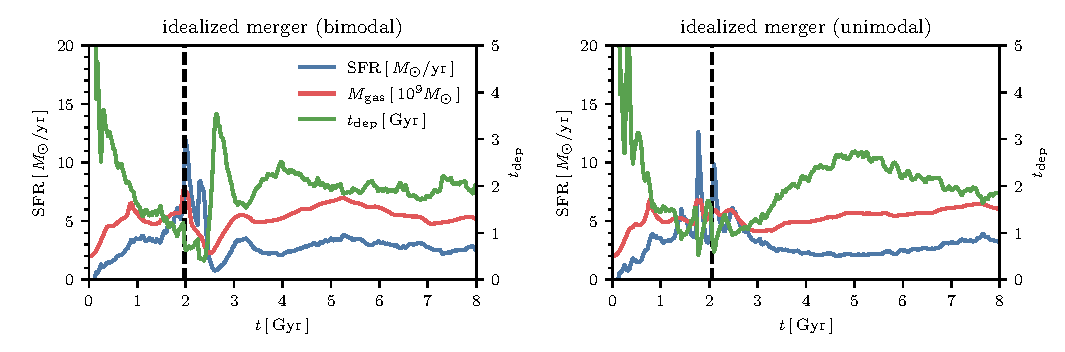
\includegraphics[width=\textwidth]{SFR_Mgas_tdep.pdf}
  \caption{\textbf{The suppression of star formation in the bimodal simulation is associated with both a reduction in gas mass as well as an increase in the depletion time.} The drop in star formation (blue line) at $\sim2.5-3\,\Gyr$ is associated with both a reduction in the total gas mass (red line) as well as an increase in the depletion time (green line). This shows that the SFR suppression is a result of both less gas mass and more inefficient star formation. \red{Should this only include the bimodal? Also, move to appendix?}}
  \label{fig:SFR_Mgas_tdep}
\end{figure*}

\begin{figure}
  \centering
  \includegraphics[width=242.26653pt]{MdotBH_rsep.pdf}
  \caption{\textbf{The bimodal merger is associated with high accretion rates onto the central SMBH.} Around the time of each pericentric passage, and slightly after, the accretion rate (blue line) becomes very high. Here, it is shown as a fraction of the Eddington accretion rate. During the merger, the accretion rate reaches as high as Eddington at some times, but is always above $10\%$. The orbital separation between the central and satellite is shown in the orange line.}
  \label{fig:MdotBH_rsep}
\end{figure}